\chapter{Reconstruction and Stripping Efficiencies}
\label{chap:stripeff}
%\chapquote{}{}
The combined reconstruction and \gls{stripping} efficiency is determined with \gls{mc} simulated events.
A full \gls{mc} simulation of a single event includes a time consuming simulation of the interactions of the particle shower with the detector material, as well as the response of the detector itself.
The reconstruction efficiency of the \lhcb detector is well below 100\,\%, \eg{}, particles with a transverse momentum below a certain threshold will almost never be stored to disk due to the associated noisy detector response, unmet trigger requirements, or geometric cut-offs.
During simulations, decays which only produce such particles are skipped to save the time intensive simulation of the detector traversal.
This so-called \textit{Generator Cut} has no counterpart in recorded data but will not change the overall efficiency when the latter is defined wide enough such that it covers selection requirements which would filter out these events for good.
For the present analysis the \gls{stripping} phase obeys this requirement such that, from a technical point of view, the product of reconstruction and \gls{stripping} efficiency is given by\footnote{Trigger decisions are only set as \textit{trigger bits} at this point and are thus not part of any selection requirement yet.}
\begin{equation}
    \label{eq:stripeff_defeps}
    \text{rec.} \times \text{strip.\ eff.} = \varepsilon_{\text{gen}} \times \frac{\texttt{\#DTT}}{\texttt{\#DST}} \,,
\end{equation}
where $\varepsilon_{\text{gen}}$ is the generator cut efficiency, and \texttt{\#DST} and \texttt{\#DTT} are technical abbreviations for the total amount of events after the detector simulation and the number of events after the respective \gls{stripping} phase.

These efficiencies are not stable during \gls{runtwo}, since (high) level triggers are under permanent changes as well as the simulation algorithms.
In Appx.~\ref{chap:apdx_stripeff} we list the trigger and simulation versions for the decays under consideration (\cf{}~Tab.~\ref{tab:apdx_simtrig}) and show graphical representations of the respective generator cut efficiencies (\cf{}~Fig.~\ref{fig:apdx_gencuteff}).
The combined reconstruction and \gls{stripping} efficiency is shown in Fig.~\ref{fig:stripeff_effs}.
The corresponding values are listed in Tab.~\ref{tab:apdx_ndstdtt1} and Tab.~\ref{tab:apdx_ndstdtt2}.
\begin{figure}[htbp]
    \centering
    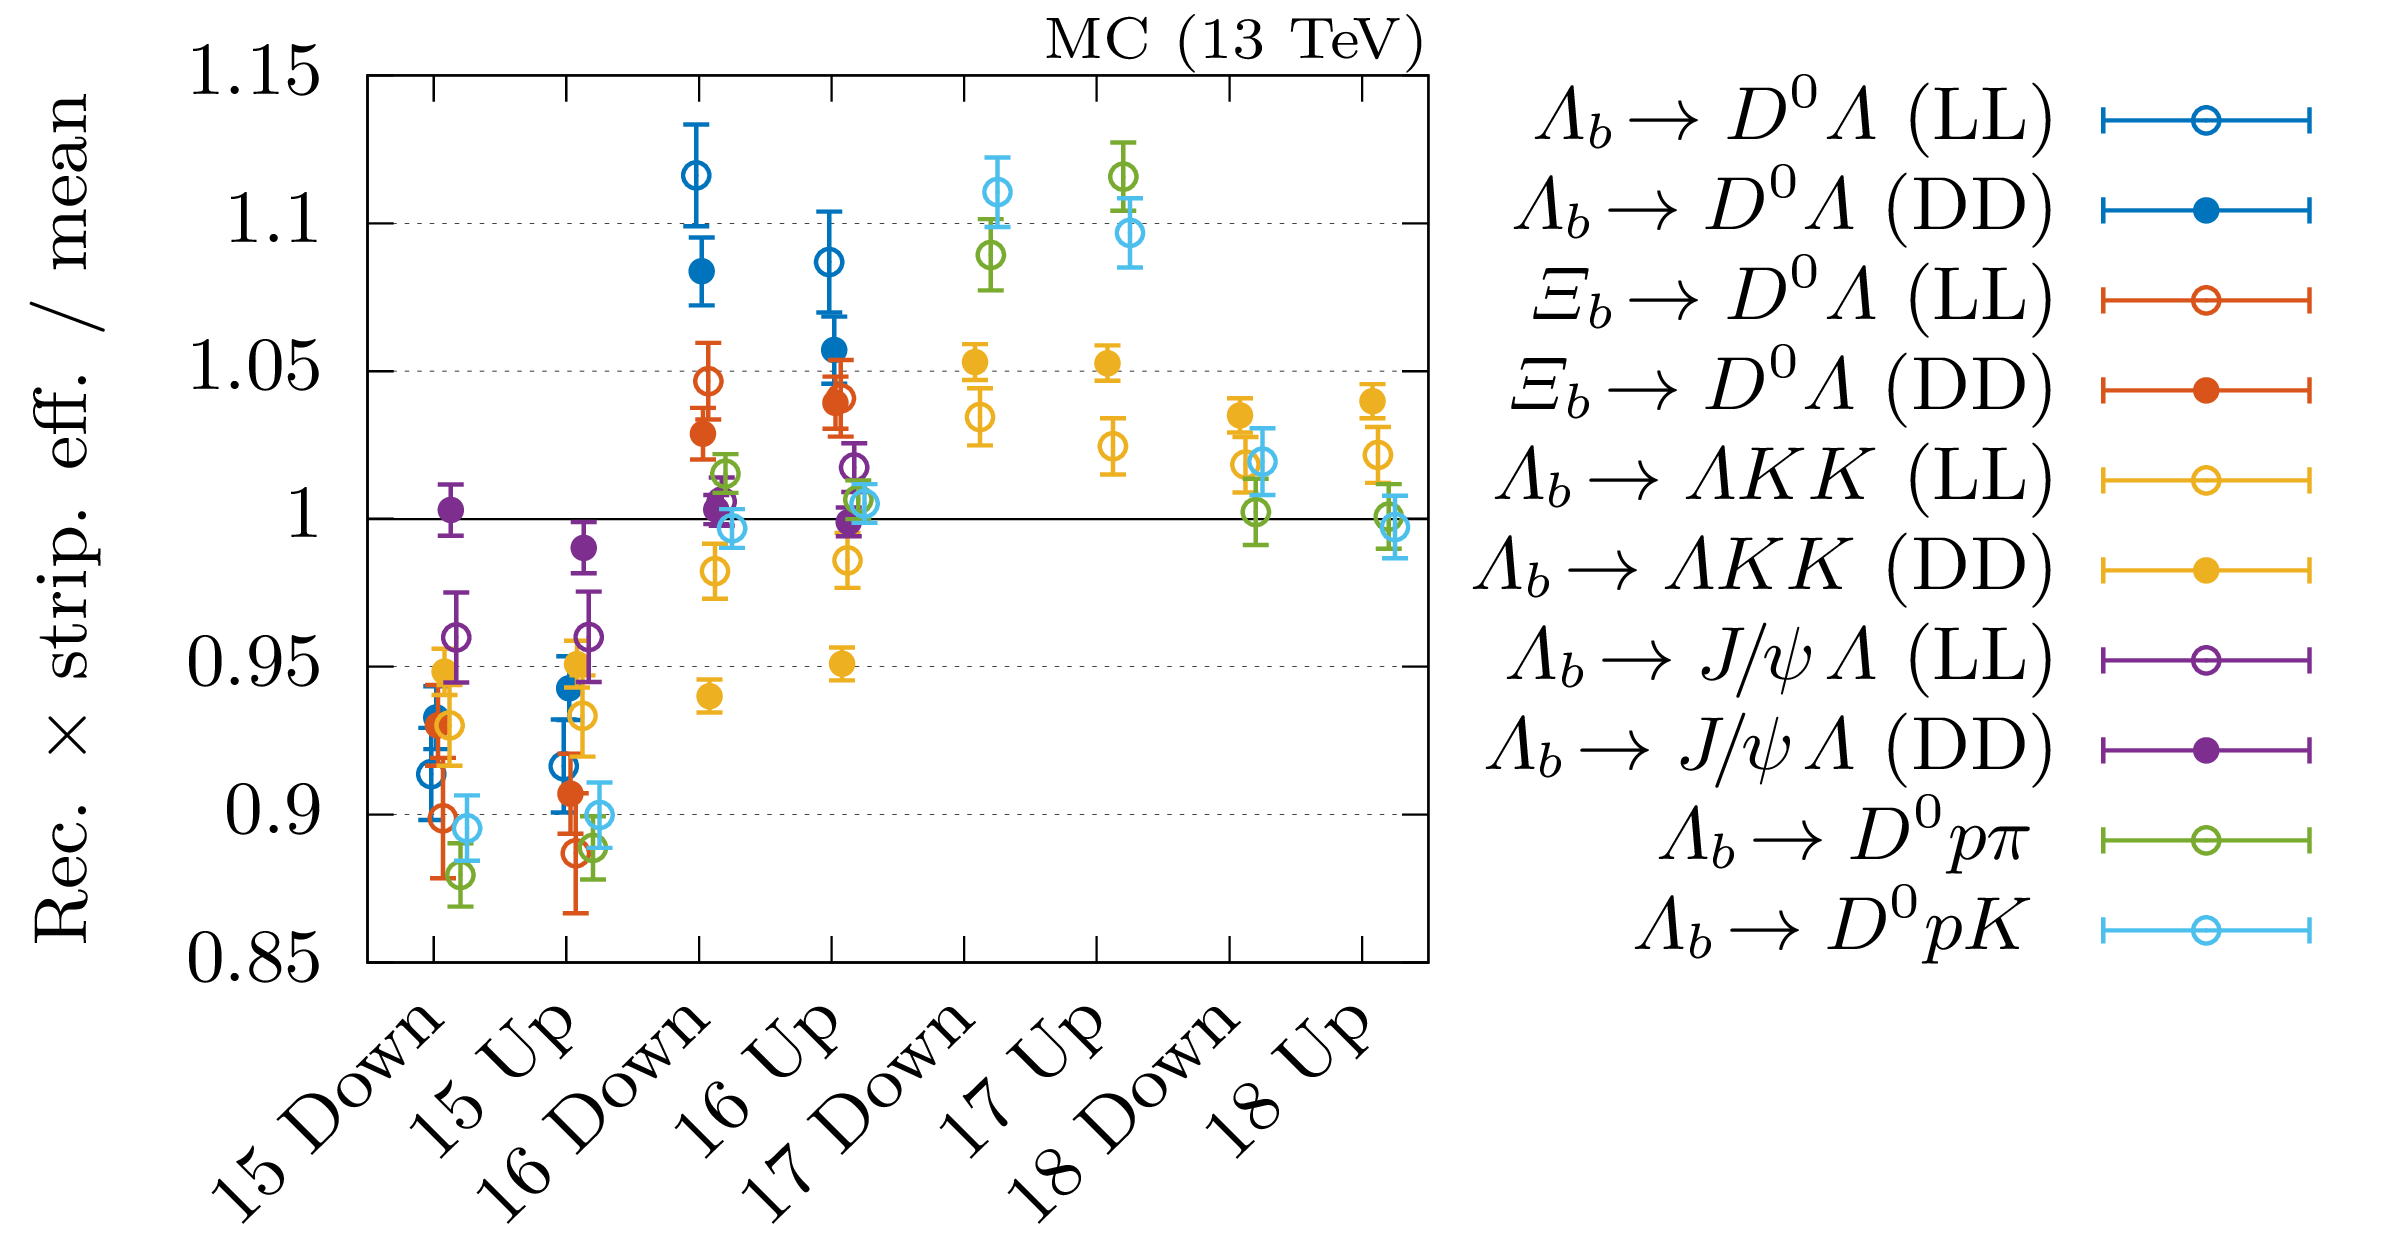
\includegraphics[scale=1.]{stripeff/effs.png}
    \caption{Combined reconstruction and \gls{stripping} efficiency for the decays under consideration. For the sake of brevity, magnet polarities are referred to as \textit{Down} and \textit{Up} for mag.\ down and mag.\ up, respectively. In order to compensate for their wide spread, each value is normalized to the respective weighted mean of each decay for the full available data set. (Not all decays are simulated for the years 2017 and 2018.) For example $y \approx 0.95$ for \decay{\Lb}{\Lz\kaon\kaon} (DD) at $x=$ 15 Down reads as a 5\,\% deviation from the weighted mean of all simulated \decay{\Lb}{\Lz\kaon\kaon} decays with \gls{DD} tracks, where $x$ and $y$ refer to the abscissa and ordinate, respectively.}
    \label{fig:stripeff_effs}
\end{figure}
The efficiencies shown in Fig.~\ref{fig:stripeff_effs} are normalized to the respective weighted mean of each decay for the full available data set (still separated w.r.t.\ the track types \gls{LL} and \gls{DD}) where we find the weighted mean $\varepsilon$ of $N$ efficiencies $p_i = n_i / N_i$ by calculating\footnote{In order to unfold relative deviations among different \gls{mc} simulated decays from biases introduced by fit models, we use \gls{truthmatched} events for this task.}
\begin{equation*}
    \varepsilon = \frac{\sum_i^N w_i \, p_i \, \varepsilon_{\text{gen},i}}{\sum_i^N w_i} \,,
\end{equation*}
where $w_i$ is the inverse sum in quadrature of the uncertainty of the generator cut efficiency $\sigma_{\text{gen},i}$ and the respective binomial uncertainty
\begin{equation*}
    w_i = \sigma_i^{-2} = \left(\sigma_{\text{gen},i}^2 + \frac{p_i (1 - p_i)}{N_i} \right)^{-1}.
\end{equation*}
Several things in Fig.~\ref{fig:stripeff_effs} are striking:
\begin{itemize}
    \item The discrepancy between simulated \decay{\Lb}{\Dz\Lz} and \decay{\Xibz}{\Dz\Lz} decays is larger than anticipated: The kinematics of both topologically identical decays should be very similar such that the deviation was more likely introduced by the various updates to the simulation framework (\texttt{Sim09c} $\to$ \texttt{Sim09h/g}). Therefore, we take simulated \decay{\Xibz}{\Dz\Lz} decays as the better proxy of genuine \decay{\Lb}{\Dz\Lz} decays than the dedicated \decay{\Lb}{\Dz\Lz} simulation for determining the combined generator cut and stripping efficiency.
    \item The efficiency drop for $\decay{\Lb}{\Dz\proton\Ph^-}$ for the year 2018: For the present analysis this drop affects \decay{\Lb}{\Dz\proton\pim} and stays unclear. For comparison we added the efficiency of \gls{mc} simulated \decay{\Lb}{\Dz\proton\Km} and \decay{\Lb}{\Lz\Kp\Km} where the drop is only visible for the former, hinting towards a correlation with the \Dz meson.
    \item The difference between \gls{LL} and \gls{DD} tracks is compatible for \decay{\Lb}{\jpsi\Lz} and \decay{\Lb}{\Lz\Kp\Km}: Even though the detector response for the former can be very different due to the dimuon pair in the final state, the difference between the track types of the \Lz daughters should be similar for the former and the latter. Further, we see that the variation of \gls{DD} tracks is smaller than for \gls{LL} tracks in both cases for the years 2015 and 2016.
    \item Similarly, the double ratio of \decay{\Lb}{\Dz\Lz} and \decay{\Xibz}{\Dz\Lz} and both track types is compatible with one. Hence, the ratio of the products of reconstruction and \gls{stripping} efficiency for \decay{\Lb}{\Dz\Lz} and \decay{\Xibz}{\Dz\Lz} does not depend on the track type in good approximation. 
\end{itemize}
The observed deviations do come with uncertainties and pinpointing exact causes is not possible.
When reliable values of the efficiencies are needed, we will therefore add a 10\,\% uncertainty to compensate for deviations that where introduced in the \gls{mc} simulated events but do not have any counterpart in recorded data.
This is a conservative approximation and will likely, based on the presented study, cover the true deviation.

%\section{Suppression Factors}
%\label{sec:stripeff_sups}
Taking the ratios of the combined reconstruction and \gls{stripping} efficiency of two \Lb decay modes gives access to suppression factors up to the \gls{stripping} process.
There are two relevant cases, first the relative suppression of \decay{\Lb}{\Dz\proton\pim} and \decay{\Lb}{\Dz\Lz}, needed for estimating the relative branching fraction of both, and secondly, the suppression of physical background contributions of \decay{\Lb}{\Dz\proton\pim} and \decay{\Lb}{\Lz\Kp\Km} in the invariant mass of \Dz and \Lz candidates.

For estimating the former, we use \gls{mc} simulated \decay{\Lb}{\Dz\proton\pim} events, reconstructed as \decay{\Lb}{\Dz\proton\pim}, and \gls{mc} simulated \decay{\Xib}{\Dz\Lz} events, reconstructed as \decay{\Lb}{\Dz\Lz} (the difference between reconstructed \Lb and \Xib is only the name tag).
The ratio as a function of different simulation conditions and track types of the \Lz daughters is shown in Fig.~\ref{fig:stripeff_Dzppi_vs_DzLz}.
\begin{figure}[htbp]
    \centering
    \begin{subfigure}{.49\textwidth}
        \centering
        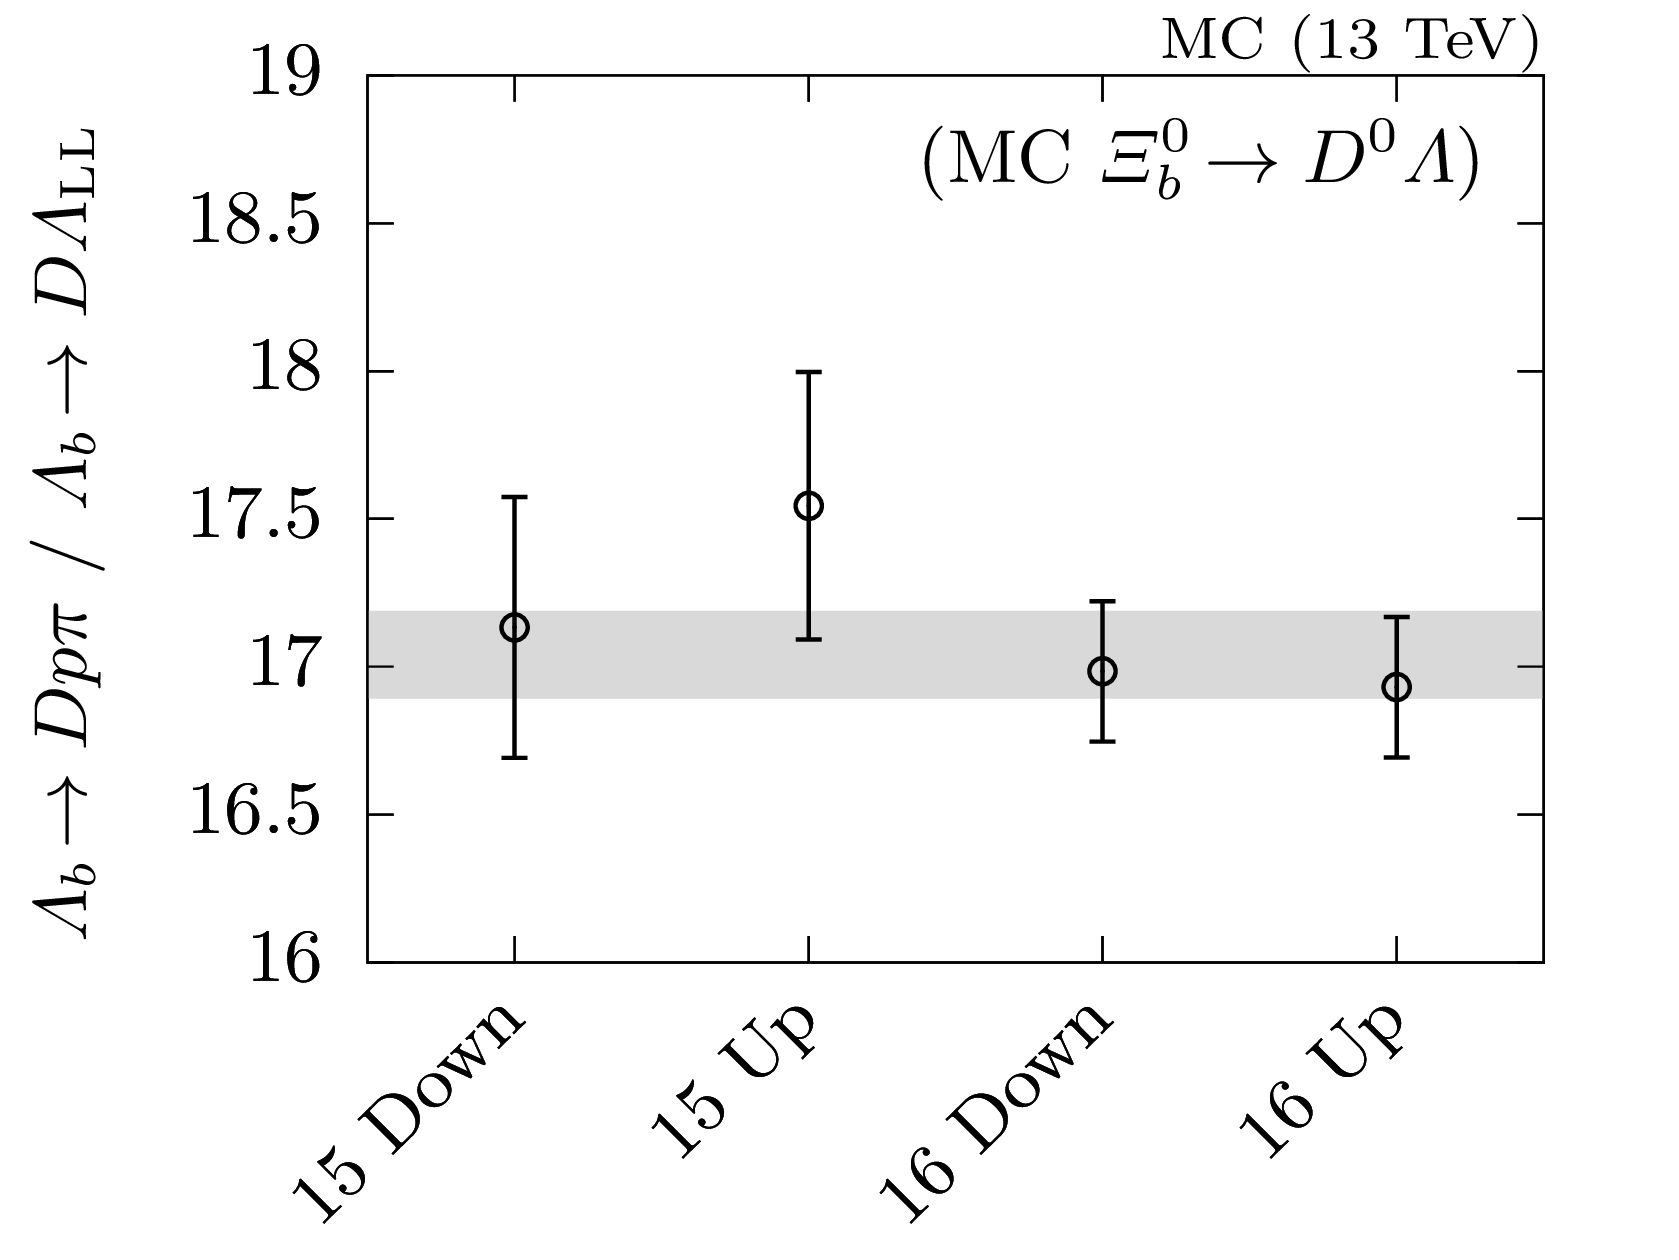
\includegraphics[scale=1.]{stripeff/ratio_Lb2Dzppi_Xib2DzLz_LL.png}
        \caption{\Lz reconstructed with \gls{LL} tracks}
    \end{subfigure}
    \begin{subfigure}{.49\textwidth}
        \centering
        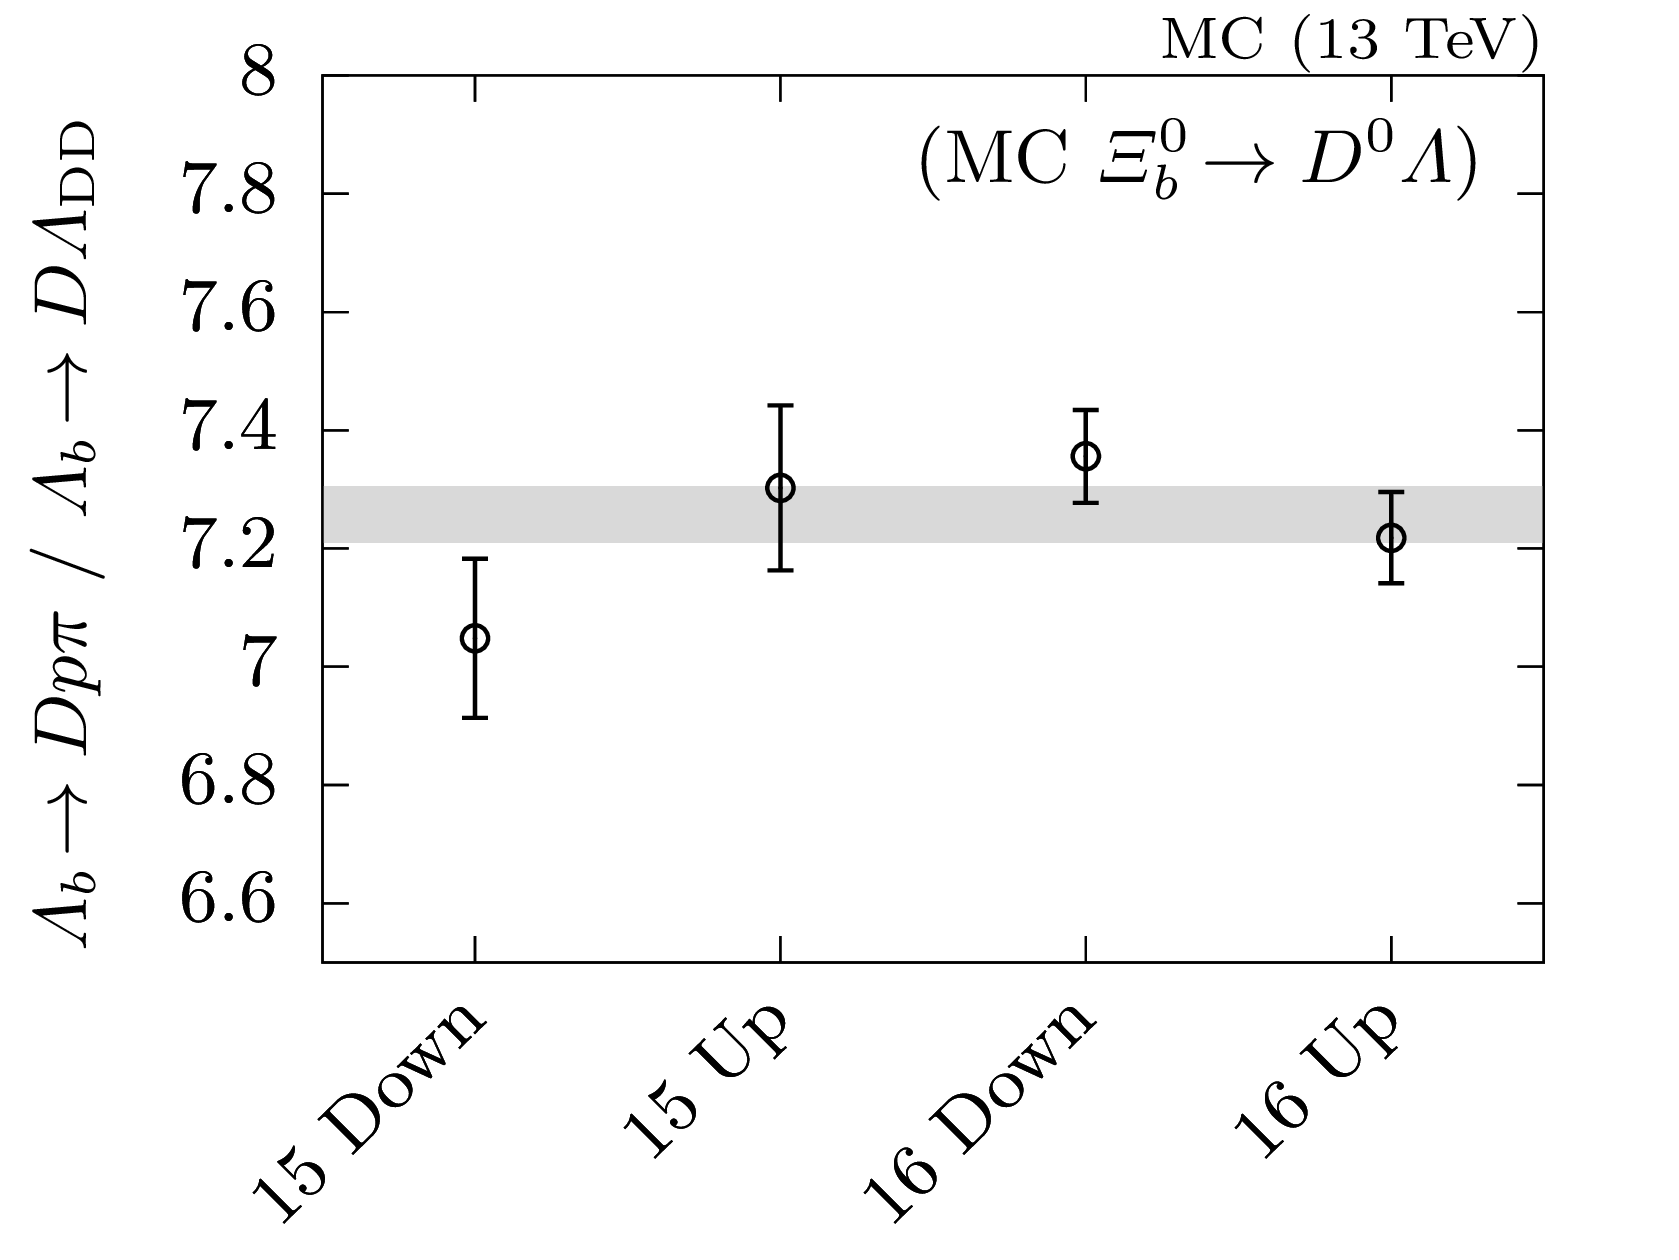
\includegraphics[scale=1.]{stripeff/ratio_Lb2Dzppi_Xib2DzLz_DD.png}
        \caption{\Lz reconstructed with \gls{DD} tracks}
    \end{subfigure}
    \caption{Ratio of the combined reconstruction and \gls{stripping} efficiency of \decay{\Lb}{\Dz\proton\pim} and \decay{\Lb}{\Dz\Lz} where we used \decay{\Xib}{\Dz\Lz} simulated decays as a proxy for the latter and differentiate between the track type of the \Lz daughters. The weighted means (grey box) are $17.04(15)$ and $7.26(5)$ for \gls{LL} tracks (left) and \gls{DD} tracks (right), respectively.}
    \label{fig:stripeff_Dzppi_vs_DzLz}
\end{figure}
The weighted means are $17.04(15)$ and $7.26(5)$ for \gls{LL} and \gls{DD} tracks, respectively.

The suppression factor $s$ of the background contribution of \decay{\Lb}{\Dz\proton\pim} in the invariant mass $m(\Dz\Lz)$ is only relevant for \gls{LL} tracks and is given by the ratio of the combined reconstruction and \gls{stripping} efficiency $\varepsilon$ of simulated \decay{\Lb}{\Dz\proton\pim} decays when reconstructed as \Dz\proton\pim and \Dz\Lz.
This suppression factor $s$ reduces the amount $n$ of reconstructed \decay{\Lb}{\Dz\proton\pim} decays, determined by an appropriate fitting technique in recorded data\footnote{In particular this means $n \neq \texttt{\#DTT}$ as used in Eq.~\eqref{eq:stripeff_defeps}.},
\begin{equation*}
    n / s = \left. n \middle/ \frac{\varepsilon\!\left( \decay{\Lb}{\Dz\proton\pim} \rightsquigarrow \Dz\proton\pim \right)}{\varepsilon\!\left( \decay{\Lb}{\Dz\proton\pim} \rightsquigarrow \Dz\Lz \right)} \right.,
\end{equation*}
where $\rightsquigarrow$ indicates the reconstruction state, hence $n/s$ is the expected amount of background contributions in $m(\Dz\Lz)$ up to the \gls{stripping} stage.

Since the recorded \decay{\Lb}{\Dz\proton\pim} sample allows a clean extraction of $n$, whereas the available samples of \decay{\Lb}{\Lz\Kp\Km} is noisier due to the smaller branching fraction and more pronounced background contributions (\cf{}~Ref.~\cite{LbToLzhh}), we also use $n$ for estimating the background contributions of charmless backgrounds.
We therefore take the results of the \gls{pdg},
\begin{align*}
    \frac{\BR(\decay{\Lb}{\Lz\Kp\Km})}{\BR(\decay{\Lb}{\Lc\pim})} &= (3.29 \pm 0.39) \times 10^{-3} \,, \\
    \frac{\BR(\decay{\Lb}{\Dz\proton\pim})}{\BR(\decay{\Lb}{\Lc\pim})} &= 0.13 \pm 0.01 \,,
\end{align*}
which are derived from the reported results of Refs.~\cite{LbToLzhh,LbToDzphAndLch}, and find
\begin{equation*}
    \kappa := \frac{\BR(\decay{\Lb}{\Dz\proton\pim})}{\BR(\decay{\Lb}{\Lz\Kp\Km})} = 40 \pm 6 \,,
\end{equation*}
assuming uncorrelated errors.
The latter assumption only holds for the statistical uncertainty strictly since both analyses are using different decay channels.
The systematic uncertainties though, do include a non-vanishing correlation, in particular because both analyses where carried out using data from the same detector.
Unfolding of correlated and uncorrelated fractions, however, is non-obvious and we will therefore use the conservative assumption of purely uncorrelated contributions which will slightly overestimate the total uncertainty.

Using $\kappa$ as the correction factor, the amount of reconstructed \decay{\Lb}{\Lz\Km\Kp} decays thus reads
\begin{equation*}
    n / s' = \left. n \middle/ \left( \kappa \times \frac{\varepsilon\!\left( \decay{\Lb}{\Dz\proton\pim} \rightsquigarrow \Dz\proton\pim \right)}{\varepsilon\!\left( \decay{\Lb}{\Lz\Km\Kp} \rightsquigarrow \Dz\Lz \right)} \times \frac{\BR(\decay{\Dz}{\Km\pip})}{\BR(\decay{\Lz}{\proton\pim})} \right) \right..
\end{equation*}
The values of $s$ and $s'$ are shown in Fig.~\ref{fig:stripeff_bkgsups}.
The weighted mean values are
\begin{subequations}
\label{eq:strip_effs_supfac}
\begin{align}
    s &= \num{24.4 \pm 0.4} \,, \\
    s' &= \begin{cases}
        \num{530 \pm 80} & \text{(\gls{LL})} \,, \\
        \num{210 \pm 30} & \text{(\gls{DD})} \,.
    \end{cases}
\end{align}
\end{subequations}

\begin{figure}[htbp]
    \centering
    \begin{subfigure}{.49\textwidth}
        \centering
        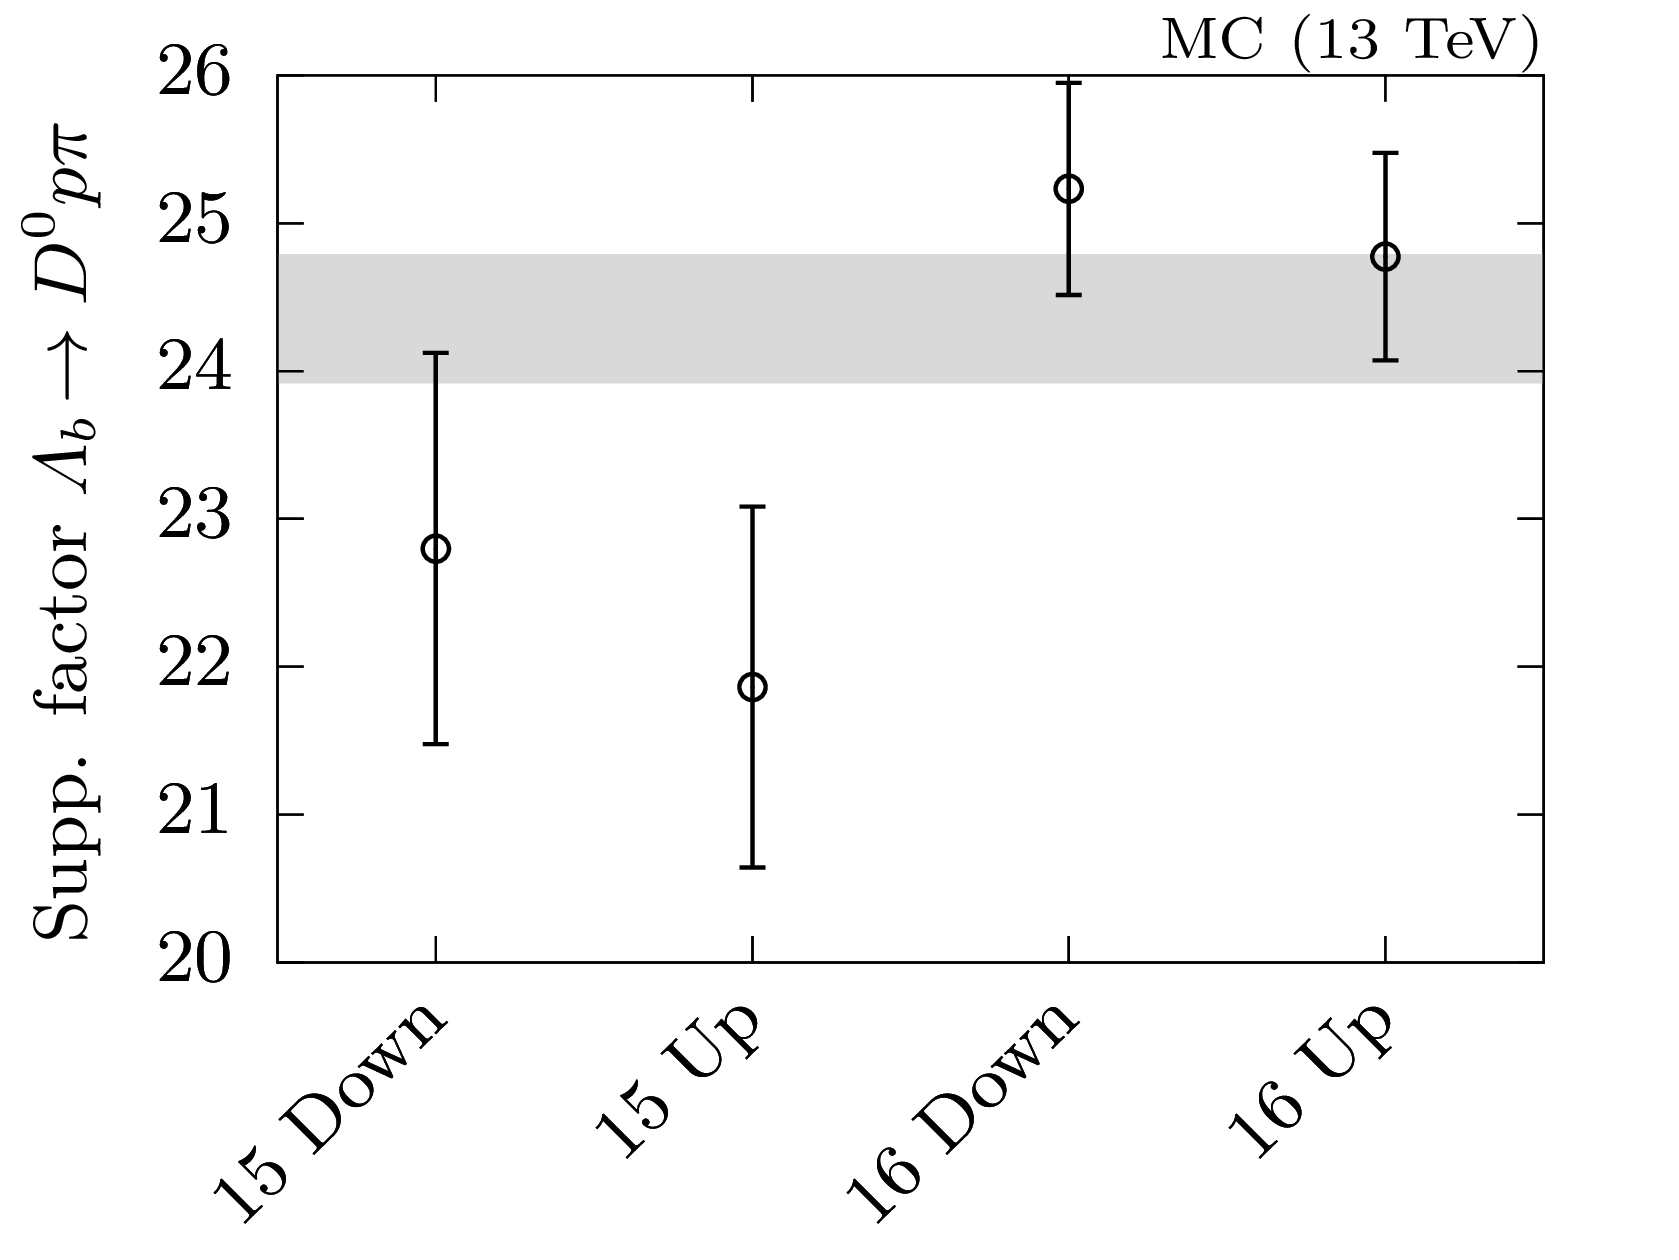
\includegraphics[scale=1.]{stripeff/bkgsup_Lb2Dzppi.png}
    \end{subfigure}
    \begin{subfigure}{.49\textwidth}
        \centering
        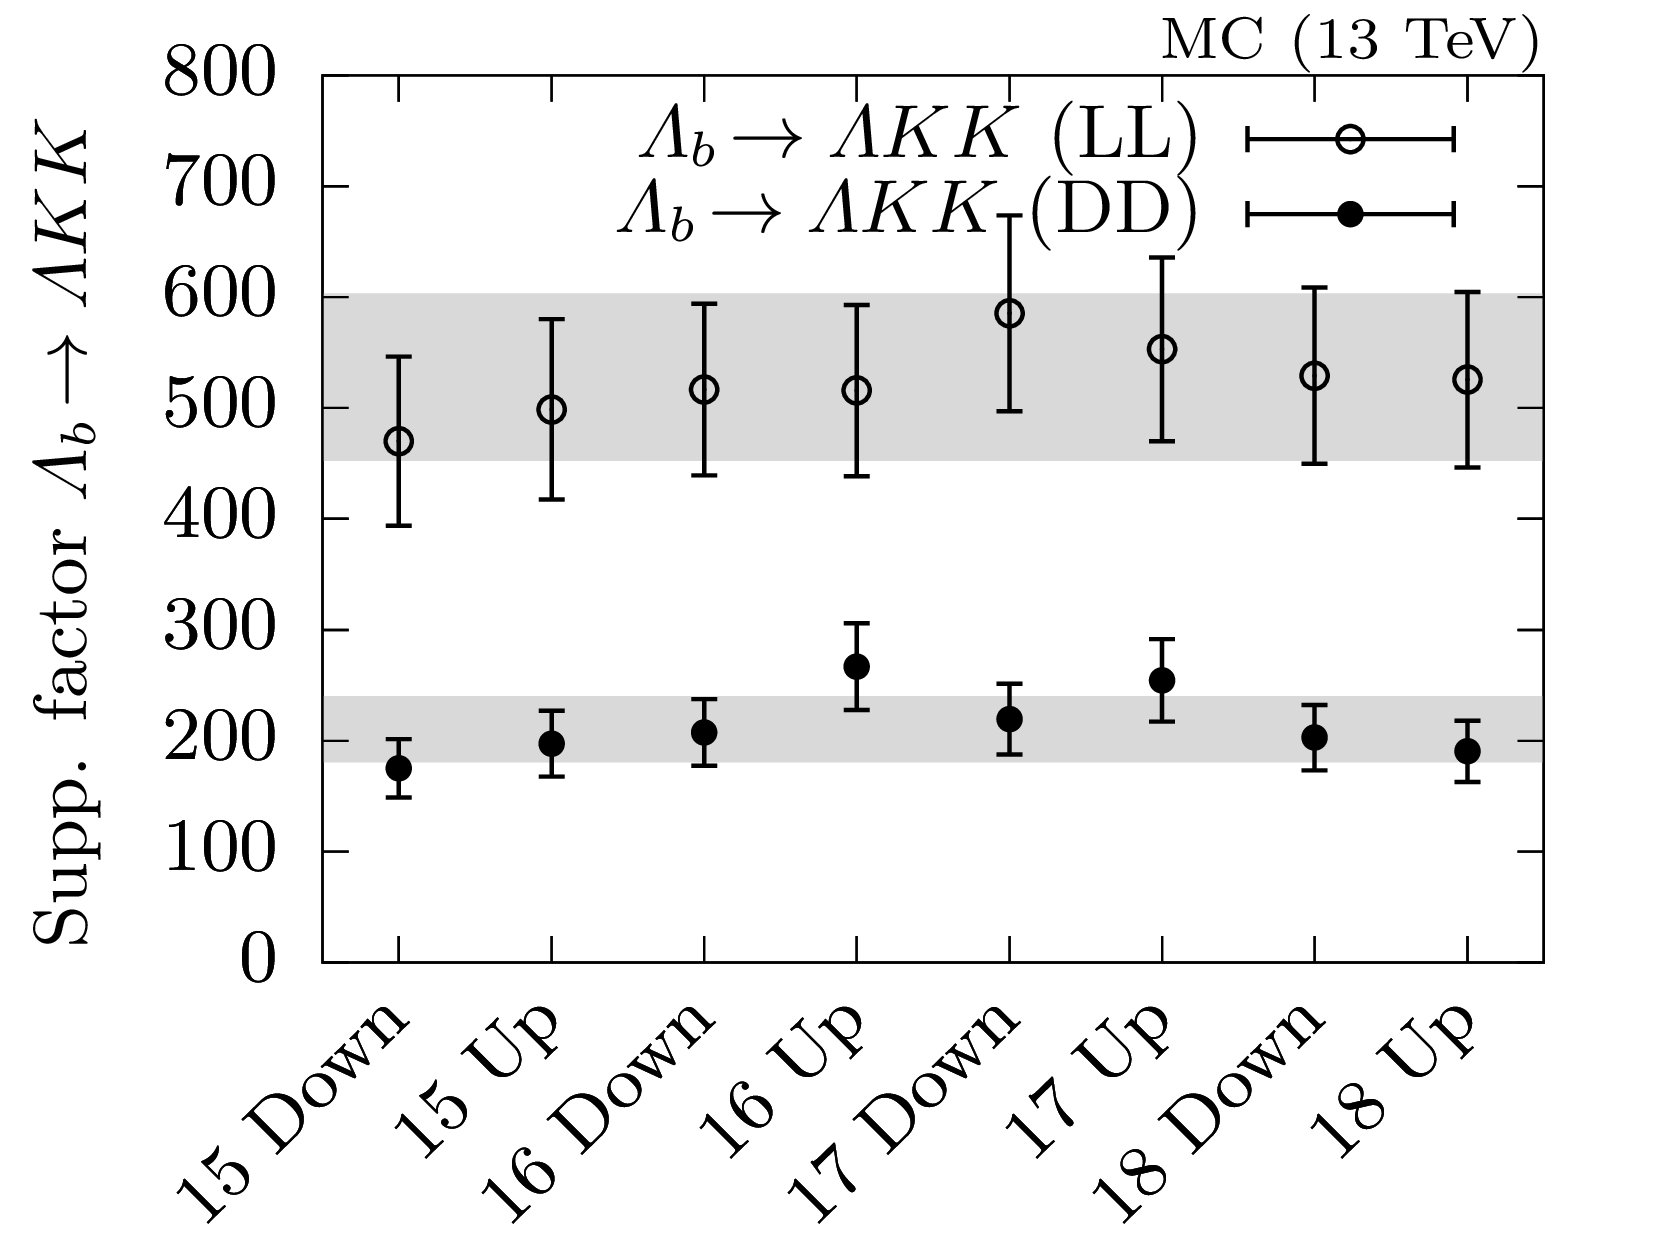
\includegraphics[scale=1.]{stripeff/bkgsup_Lb2LzKK.png}
    \end{subfigure}
    \caption{Suppression factors $s$ (left) and $s'$ (right) as defined in Eqs.~\eqref{eq:strip_effs_supfac} and respective weighted mean values (box).}
    \label{fig:stripeff_bkgsups}
\end{figure}
